\chapter{自旋系统中的拓扑}

\section{一维反铁磁海森堡自旋链}

\subsection{低能有效理论和拓扑相}

\begin{back}{自旋的路径积分}{spin-path-integral}
    自旋是可以使用路径积分描述的。这里的路径积分和通常的场论的路径积分不同,因为此时的基本自由度是自旋,没有形如$\comm*{x}{p} = \ii$这样的对易关系。
    虽然如此,我们仍然可以有路径积分,因为我们有“对自旋构型的积分”——$SU(2)$上的Haar测度——并且实际上也有“自旋相干态”。
    首先,我们知道$SU(2)$群的任何一个有限维不可约表示均可以使用如下的欧拉角表示出来:
    \begin{equation}
        g(\phi, \theta, \psi) = \ee^{- \ii \phi S_3} \ee^{- \ii \theta S_2} \ee^{- \ii \psi S_3}, \quad \phi, \psi \in [0, 2\pi], \ \theta \in [0, \pi].
    \end{equation}
    设$\ket*{\uparrow}$为$S_3$的最高权本征态,即本征值最大的本征态,我们就有
    \begin{equation}
        \ee^{- \ii \psi S_3} \ket*{\uparrow} = \ee^{- \ii \psi S} \ket*{\uparrow},
    \end{equation}
    其中$S$是$S_3$的最大本征值,对自旋$1/2$表示它是$1/2$,对自旋$1$表示它是$1$,等等。
    我们注意到
    \[
        \begin{aligned}
            \ii \mel*{\uparrow}{S_2}{\uparrow} &= \mel*{\uparrow}{\comm*{S_3}{S_1}}{\uparrow} \\
            &= S \mel*{\uparrow}{S_1}{\uparrow} - S \mel*{\uparrow}{S_1}{\uparrow} = 0,
        \end{aligned}
    \]
    同理
    \[
        \mel*{\uparrow}{S_1}{\uparrow} = 0.
    \]
    定义
    \begin{equation}
        \ket*{g} = g \ket*{\uparrow}, \quad g \in SU(2),
    \end{equation}
    称它为\concept{自旋相干态}。这个说法的依据在于,根据Haar测度的定义,有
    \[
        h \int \dd{g} \dyad{g} = \int \dd{g} \dyad*{hg}{g} = \int \dd{g} \dyad*{g}{h^{-1} g} = \int \dd{g} \dyad{g} h, 
    \]
    根据不可约表示的Schur引理,我们有
    \begin{equation}
        \int \dd{g} \dyad{g} = \const \times \mathrm{id}, 
    \end{equation}
    得到了定义路径积分需要的完备性关系,而$\ket*{g}$的地位和基于$\vb*{x}, \vb*{p}$的路径积分中的相干态类似。
    使用“将时间分片并插入完备性关系”的方法,就有
    \begin{equation}
        Z = \int \fd{g} \exp(\int_0^\beta \dd{\tau} (\braket*{\partial_\tau g}{g} - \mel*{g}{H}{g})).
        \label{eq:spin-partition-original}
    \end{equation}
    在这里我们可以看到,自旋的路径积分只涉及一类算符($\vb*{S}$的各个分量)而不是两类($\vb*{x}$和$\vb*{p}$),从而相干态路径积分看起来会简单一些;但是自旋的路径积分中$\vb*{S}$是在一个球上取值而不是在平直的坐标空间和动量空间中取值,并且彼此不对易,因此下面当我们把这些内积展开时又会有比坐标-动量路径积分更复杂的东西。

    用欧拉角把$\ket*{g}$写出来就是
    \[
        \ket*{g} = \ee^{- \ii \psi S} \ee^{- \ii \phi S_3} \ee^{- \ii \theta S_2} \ket*{\uparrow}.
    \]
    我们首先处理\eqref{eq:spin-partition-original}的第一项,我们有
    \[
        \int_0^\beta \dd{\tau} \braket*{\partial_\tau g}{g} = \int_0^\beta \dd{\tau} (\ii S \partial_\tau \psi + \mel*{\uparrow}{\partial_\tau (\ee^{\ii \theta S_2} \ee^{\ii \phi S_3}) \ee^{- \ii \phi S_3} \ee^{- \ii \theta S_2}}{\uparrow} ),
    \]
    其中的第一项是零,因为$\psi$在$\tau = 0$和$\tau = \beta$处是相同的。
    第二项是
    \[
        \begin{aligned}
            \int_0^\beta \dd{\tau} \mel*{\uparrow}{\partial_\tau (\ee^{\ii \theta S_2} \ee^{\ii \phi S_3}) \ee^{- \ii \phi S_3} \ee^{- \ii \theta S_2}}{\uparrow} &= \int_0^\beta \dd{\tau} \ii \partial_\tau \theta \mel*{\uparrow}{S_2 \ee^{\ii \theta S_2} \ee^{\ii \phi S_3} \ee^{- \ii \phi S_3} \ee^{- \ii \theta S_2}}{\uparrow} \\
            &\quad + \int_0^\beta \dd{\tau} \mel*{\uparrow}{\ee^{\ii \theta S_2} \ii \partial_\tau \phi S_3 \ee^{\ii \phi S_3} \ee^{- \ii \phi S_3} \ee^{- \ii \theta S_2}}{\uparrow},
        \end{aligned}
    \]
    这里的第一项还是零,因为$\mel*{\uparrow}{S_2}{\uparrow}$是零。
    第二项是
    \[
        \begin{aligned}
            \int_0^\beta \dd{\tau} \mel*{\uparrow}{\ee^{\ii \theta S_2} \ii \partial_\tau \phi S_3 \ee^{\ii \phi S_3} \ee^{- \ii \phi S_3} \ee^{- \ii \theta S_2}}{\uparrow} &= \int_0^\beta \dd{\tau} \ii \partial_\tau \phi \mel*{\uparrow}{\ee^{\ii \theta S_2} S_3 \ee^{- \ii \theta S_2}}{\uparrow} \\
            &= \ii S \int_0^\beta \dd{\tau} \partial_\tau \phi \cos \theta,
        \end{aligned}
    \]
    这里我们用到了
    \[
        \begin{aligned}
            \mel*{\uparrow}{\ee^{\ii \theta S_2} S_3 \ee^{- \ii \theta S_2}}{\uparrow} &= \mel*{\uparrow}{\ee^{\ii \theta [S_2, \ ]} S_3}{\uparrow} \\
            &= \mel*{\uparrow}{1 + (\ii \theta) \ii S_1 + \frac{(\ii \theta)^2 + \cdots}{2} S_3 }{\uparrow} \\
            &= \mel*{\uparrow}{1 - \frac{\theta^2}{2} S + \cdots}{\uparrow} = S \cos \theta, 
        \end{aligned}
    \]
    因此我们有
    \begin{equation}
        \int_0^\beta \dd{\tau} \braket*{\partial_\tau g}{g} = \ii S \int_0^\beta \dd{\tau} \partial_\tau \phi \cos \theta.
    \end{equation}

    然后我们计算$\mel*{g}{H}{g}$,它基本上是$\vb*{S}$的线性函数加上某个常数项,因为自旋是矢量,而$H$是标量,因此$\vb*{S}$出现在$H$中的方式不是和某个另外的矢量点乘就是和自己点乘,或者是以上两者的多项式。
    在一个不可约表示中$\vb*{S}^2 = S(S+1)$,是常数,因此$H$是$\vb*{B} \cdot \vb*{S}$的函数,其中$\vb*{B}$是某个矢量。
    \[
        \begin{aligned}
            \mel*{g}{S_i}{g} &= \mel*{\uparrow}{\ee^{\ii \theta S_2} \ee^{\ii \phi S_3} S_i \ee^{- \ii \phi S_3} \ee^{- \ii \theta S_2}}{\uparrow}
        \end{aligned}
    \]
    这里我们用到了更加一般的
    % TODO:BS^2这种怎么办?

    \begin{equation}
        S[\theta, \phi] = S \int_0^\beta \dd{\tau} (B \cos \theta + \ii (1 - \cos \theta) \partial_\tau \phi).
        \label{eq:spin-path-integral}
    \end{equation}
    最终,$\psi$没有出现在路径积分中。我们可以用单位矢量$\vb*{n}$表示$(\theta, \phi)$在球坐标系中确定的$\vb*{S}$指向。
\end{back}

考虑一维反铁磁海森堡自旋链
\begin{equation}
    H = J \sum_{i} \vb*{S}_i \cdot \vb*{S}_{i+1}, \quad J > 0,
\end{equation}
其自旋路径积分表述为(下面注意区分作用量$S$和自旋长度$S$)
\begin{equation}
    Z = \int \prod_i \fd{\vb*{n}_i} \ee^{-S[\{\vb*{n}_i\}]} , \quad S[\{\vb*{n}_i\}] = \int \dd{\tau} \sum_i ( \ii S (1 - \cos \theta_i) \partial_\tau \phi_i + J S^2 \vb*{n}_i \cdot \vb*{n}_{i+1} ).
\end{equation}

\begin{figure}
    \centering
    \subfigure[单自旋的场构型,对应$S^2$上的曲线$\gamma$]{
        

\tikzset{every picture/.style={line width=0.75pt}} %set default line width to 0.75pt        

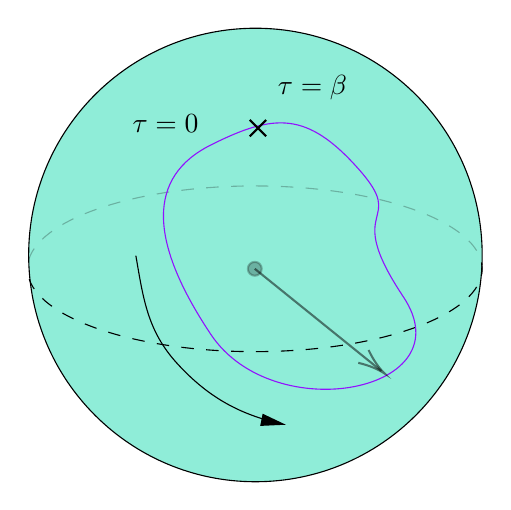
\begin{tikzpicture}[x=0.75pt,y=0.75pt,yscale=-1,xscale=1]
%uncomment if require: \path (0,300); %set diagram left start at 0, and has height of 300

%Shape: Circle [id:dp4271001416525375] 
\draw  [fill={rgb, 255:red, 80; green, 227; blue, 194 }  ,fill opacity=0.64 ] (100.21,156.46) .. controls (100.21,96.12) and (149.12,47.21) .. (209.46,47.21) .. controls (269.79,47.21) and (318.71,96.12) .. (318.71,156.46) .. controls (318.71,216.79) and (269.79,265.71) .. (209.46,265.71) .. controls (149.12,265.71) and (100.21,216.79) .. (100.21,156.46) -- cycle ;
%Shape: Arc [id:dp5416427461491542] 
\draw  [draw opacity=0][dash pattern={on 4.5pt off 4.5pt}] (318.45,160.4) .. controls (318.62,161.29) and (318.7,162.19) .. (318.7,163.09) .. controls (318.7,185.14) and (269.66,203.02) .. (209.16,203.03) .. controls (153.32,203.04) and (107.23,187.82) .. (100.46,168.14) -- (209.15,163.11) -- cycle ; \draw  [dash pattern={on 4.5pt off 4.5pt}] (318.45,160.4) .. controls (318.62,161.29) and (318.7,162.19) .. (318.7,163.09) .. controls (318.7,185.14) and (269.66,203.02) .. (209.16,203.03) .. controls (153.32,203.04) and (107.23,187.82) .. (100.46,168.14) ;
%Shape: Arc [id:dp27514417350783926] 
\draw  [draw opacity=0][dash pattern={on 4.5pt off 4.5pt}] (318.45,165.82) .. controls (318.62,164.93) and (318.7,164.03) .. (318.7,163.13) .. controls (318.7,141.08) and (269.66,123.2) .. (209.16,123.19) .. controls (153.32,123.18) and (107.23,138.4) .. (100.46,158.08) -- (209.15,163.11) -- cycle ; \draw  [color={rgb, 255:red, 0; green, 0; blue, 0 }  ,draw opacity=0.25 ][dash pattern={on 4.5pt off 4.5pt}] (318.45,165.82) .. controls (318.62,164.93) and (318.7,164.03) .. (318.7,163.13) .. controls (318.7,141.08) and (269.66,123.2) .. (209.16,123.19) .. controls (153.32,123.18) and (107.23,138.4) .. (100.46,158.08) ;
%Shape: Polygon Curved [id:ds05822553982795253] 
\draw  [color={rgb, 255:red, 144; green, 19; blue, 254 }  ,draw opacity=1 ] (187.96,103.47) .. controls (218.36,88.26) and (234.23,87.07) .. (258.97,114.83) .. controls (283.71,142.58) and (250.3,130.97) .. (280.71,176.58) .. controls (311.11,222.2) and (218.36,240.31) .. (187.96,194.69) .. controls (157.55,149.08) and (157.55,118.67) .. (187.96,103.47) -- cycle ;
%Straight Lines [id:da6134231895751854] 
\draw [color={rgb, 255:red, 0; green, 0; blue, 0 }  ,draw opacity=1 ]   (210.68,95.34) ;
\draw [shift={(210.68,95.34)}, rotate = 45] [color={rgb, 255:red, 0; green, 0; blue, 0 }  ,draw opacity=1 ][line width=0.75]    (-5.59,0) -- (5.59,0)(0,5.59) -- (0,-5.59)   ;
%Straight Lines [id:da9066706253629926] 
\draw [color={rgb, 255:red, 0; green, 0; blue, 0 }  ,draw opacity=0.5 ][line width=0.75]    (270.15,212.33) -- (209.15,163.11) ;
\draw [shift={(271.71,213.58)}, rotate = 218.9] [color={rgb, 255:red, 0; green, 0; blue, 0 }  ,draw opacity=0.5 ][line width=0.75]    (13.12,-3.95) .. controls (8.34,-1.68) and (3.97,-0.36) .. (0,0) .. controls (3.97,0.36) and (8.34,1.68) .. (13.12,3.95)   ;
%Straight Lines [id:da5443690821222467] 
\draw    (100,149.66) ;
%Straight Lines [id:da23851388151552166] 
\draw [color={rgb, 255:red, 0; green, 0; blue, 0 }  ,draw opacity=0.25 ]   (209.15,163.11) ;
\draw [shift={(209.15,163.11)}, rotate = 0] [color={rgb, 255:red, 0; green, 0; blue, 0 }  ,draw opacity=0.25 ][fill={rgb, 255:red, 0; green, 0; blue, 0 }  ,fill opacity=0.25 ][line width=0.75]      (0, 0) circle [x radius= 3.35, y radius= 3.35]   ;
%Curve Lines [id:da94729558266777] 
\draw    (151.85,156.78) .. controls (155.41,177.15) and (157.29,192.83) .. (171.61,208.56) .. controls (185.57,223.89) and (200.71,233.21) .. (222.42,237.89) ;
\draw [shift={(224.11,238.24)}, rotate = 191.4] [fill={rgb, 255:red, 0; green, 0; blue, 0 }  ][line width=0.08]  [draw opacity=0] (12,-3) -- (0,0) -- (12,3) -- cycle    ;

% Text Node
\draw (149,87.4) node [anchor=north west][inner sep=0.75pt]    {$\tau =0$};
% Text Node
\draw (219,68.4) node [anchor=north west][inner sep=0.75pt]    {$\tau =\beta $};


\end{tikzpicture}

        \label{fig:spin-field-configuration}
    }
    \subfigure[路径积分中的$(1 - \cos \theta) \partial_\tau \phi$微元]{
        

\tikzset{every picture/.style={line width=0.75pt}} %set default line width to 0.75pt        

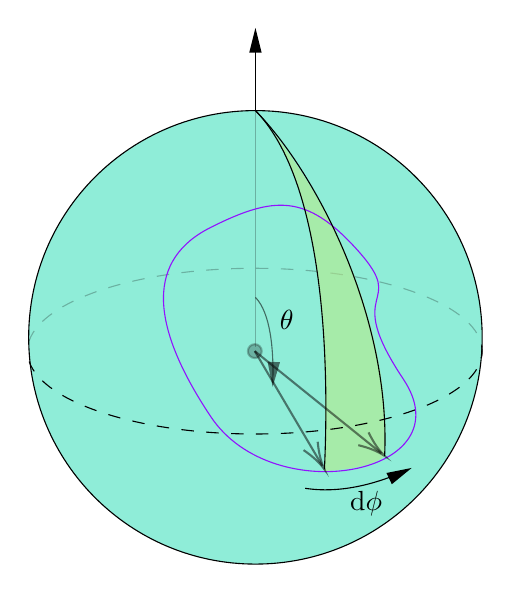
\begin{tikzpicture}[x=0.75pt,y=0.75pt,yscale=-1,xscale=1]
%uncomment if require: \path (0,300); %set diagram left start at 0, and has height of 300

%Shape: Circle [id:dp13786767435744185] 
\draw  [fill={rgb, 255:red, 80; green, 227; blue, 194 }  ,fill opacity=0.64 ] (337.21,163.46) .. controls (337.21,103.12) and (386.12,54.21) .. (446.46,54.21) .. controls (506.79,54.21) and (555.71,103.12) .. (555.71,163.46) .. controls (555.71,223.79) and (506.79,272.71) .. (446.46,272.71) .. controls (386.12,272.71) and (337.21,223.79) .. (337.21,163.46) -- cycle ;
%Shape: Arc [id:dp9522431051366946] 
\draw  [draw opacity=0][dash pattern={on 4.5pt off 4.5pt}] (555.45,172.82) .. controls (555.62,171.93) and (555.7,171.03) .. (555.7,170.13) .. controls (555.7,148.08) and (506.66,130.2) .. (446.16,130.19) .. controls (390.32,130.18) and (344.23,145.4) .. (337.46,165.08) -- (446.15,170.11) -- cycle ; \draw  [color={rgb, 255:red, 0; green, 0; blue, 0 }  ,draw opacity=0.25 ][dash pattern={on 4.5pt off 4.5pt}] (555.45,172.82) .. controls (555.62,171.93) and (555.7,171.03) .. (555.7,170.13) .. controls (555.7,148.08) and (506.66,130.2) .. (446.16,130.19) .. controls (390.32,130.18) and (344.23,145.4) .. (337.46,165.08) ;
%Shape: Polygon Curved [id:ds20966219878034242] 
\draw  [draw opacity=0][fill={rgb, 255:red, 184; green, 233; blue, 134 }  ,fill opacity=0.57 ] (446.46,54.21) .. controls (499.46,116.46) and (511.46,182.1) .. (508.71,220.58) .. controls (504.36,224.5) and (495.56,226.7) .. (479.76,227.9) .. controls (479.96,197.7) and (485.06,94.06) .. (446.46,54.21) -- cycle ;
%Straight Lines [id:da040656680856383076] 
\draw    (446.46,16.32) -- (446.46,54.21) ;
\draw [shift={(446.46,14.32)}, rotate = 90] [fill={rgb, 255:red, 0; green, 0; blue, 0 }  ][line width=0.08]  [draw opacity=0] (12,-3) -- (0,0) -- (12,3) -- cycle    ;
%Straight Lines [id:da786719038701464] 
\draw [color={rgb, 255:red, 0; green, 0; blue, 0 }  ,draw opacity=0.25 ]   (446.46,54.21) -- (446.46,168.23) ;
%Shape: Arc [id:dp9443167576463041] 
\draw  [draw opacity=0][dash pattern={on 4.5pt off 4.5pt}] (555.45,167.4) .. controls (555.62,168.29) and (555.7,169.19) .. (555.7,170.09) .. controls (555.7,192.14) and (506.66,210.02) .. (446.16,210.03) .. controls (390.32,210.04) and (344.23,194.82) .. (337.46,175.14) -- (446.15,170.11) -- cycle ; \draw  [dash pattern={on 4.5pt off 4.5pt}] (555.45,167.4) .. controls (555.62,168.29) and (555.7,169.19) .. (555.7,170.09) .. controls (555.7,192.14) and (506.66,210.02) .. (446.16,210.03) .. controls (390.32,210.04) and (344.23,194.82) .. (337.46,175.14) ;
%Shape: Polygon Curved [id:ds8135273243457903] 
\draw  [color={rgb, 255:red, 144; green, 19; blue, 254 }  ,draw opacity=1 ] (424.96,110.47) .. controls (455.36,95.26) and (471.23,94.07) .. (495.97,121.83) .. controls (520.71,149.58) and (487.3,137.97) .. (517.71,183.58) .. controls (548.11,229.2) and (455.36,247.31) .. (424.96,201.69) .. controls (394.55,156.08) and (394.55,125.67) .. (424.96,110.47) -- cycle ;
%Straight Lines [id:da0919823888859701] 
\draw [color={rgb, 255:red, 0; green, 0; blue, 0 }  ,draw opacity=0.5 ][line width=0.75]    (507.15,219.33) -- (446.15,170.11) ;
\draw [shift={(508.71,220.58)}, rotate = 218.9] [color={rgb, 255:red, 0; green, 0; blue, 0 }  ,draw opacity=0.5 ][line width=0.75]    (13.12,-3.95) .. controls (8.34,-1.68) and (3.97,-0.36) .. (0,0) .. controls (3.97,0.36) and (8.34,1.68) .. (13.12,3.95)   ;
%Straight Lines [id:da7641038914794658] 
\draw    (337,156.66) ;
%Straight Lines [id:da8631491702531824] 
\draw [color={rgb, 255:red, 0; green, 0; blue, 0 }  ,draw opacity=0.25 ]   (446.15,170.11) ;
\draw [shift={(446.15,170.11)}, rotate = 0] [color={rgb, 255:red, 0; green, 0; blue, 0 }  ,draw opacity=0.25 ][fill={rgb, 255:red, 0; green, 0; blue, 0 }  ,fill opacity=0.25 ][line width=0.75]      (0, 0) circle [x radius= 3.35, y radius= 3.35]   ;
%Straight Lines [id:da12016344147570801] 
\draw [color={rgb, 255:red, 0; green, 0; blue, 0 }  ,draw opacity=0.5 ][line width=0.75]    (478.69,225.36) -- (446.15,170.11) ;
\draw [shift={(479.71,227.09)}, rotate = 239.51] [color={rgb, 255:red, 0; green, 0; blue, 0 }  ,draw opacity=0.5 ][line width=0.75]    (13.12,-3.95) .. controls (8.34,-1.68) and (3.97,-0.36) .. (0,0) .. controls (3.97,0.36) and (8.34,1.68) .. (13.12,3.95)   ;
%Curve Lines [id:da7960637854392238] 
\draw    (470.4,236.19) .. controls (490.04,239.21) and (508.96,232.26) .. (520.04,227.17) ;
\draw [shift={(521.73,226.38)}, rotate = 514.62] [fill={rgb, 255:red, 0; green, 0; blue, 0 }  ][line width=0.08]  [draw opacity=0] (12,-3) -- (0,0) -- (12,3) -- cycle    ;
%Curve Lines [id:da46076484070564927] 
\draw    (446.46,54.21) .. controls (476.71,85.2) and (482.71,161.2) .. (479.71,227.09) ;
%Curve Lines [id:da07397623956465105] 
\draw    (446.46,54.21) .. controls (476.71,85.2) and (511.71,154.69) .. (508.71,220.58) ;
%Curve Lines [id:da7251628481913182] 
\draw [color={rgb, 255:red, 0; green, 0; blue, 0 }  ,draw opacity=0.54 ]   (446.46,144.2) .. controls (453.7,151.61) and (455.36,169.37) .. (454.82,185.31) ;
\draw [shift={(454.75,187.3)}, rotate = 272.61] [fill={rgb, 255:red, 0; green, 0; blue, 0 }  ,fill opacity=0.54 ][line width=0.08]  [draw opacity=0] (12,-3) -- (0,0) -- (12,3) -- cycle    ;

% Text Node
\draw (457,149.4) node [anchor=north west][inner sep=0.75pt]    {$\theta $};
% Text Node
\draw (499.79,236.4) node [anchor=north] [inner sep=0.75pt]    {$\mathrm{d} \phi $};


\end{tikzpicture}

    }
    \subfigure[单自旋的场构型,对应$S^2$上的曲线$\gamma$]{
        

\tikzset{every picture/.style={line width=0.75pt}} %set default line width to 0.75pt        

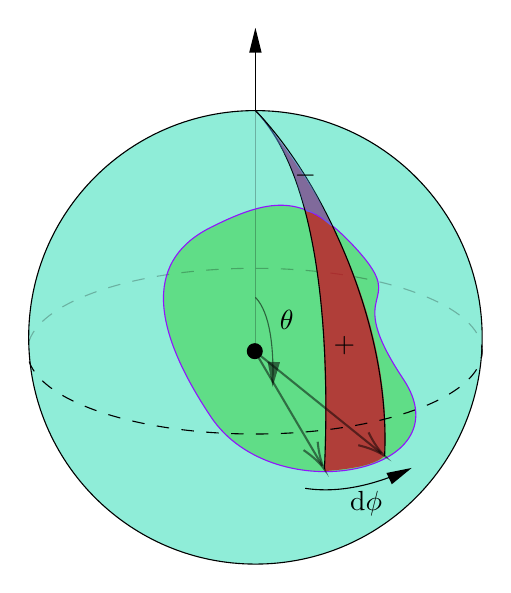
\begin{tikzpicture}[x=0.75pt,y=0.75pt,yscale=-1,xscale=1]
%uncomment if require: \path (0,300); %set diagram left start at 0, and has height of 300

%Shape: Polygon Curved [id:ds889444292321216] 
\draw  [draw opacity=0][fill={rgb, 255:red, 126; green, 211; blue, 33 }  ,fill opacity=1 ] (349.96,114.76) .. controls (380.36,99.55) and (396.23,98.36) .. (420.97,126.12) .. controls (445.71,153.88) and (412.3,142.26) .. (442.71,187.88) .. controls (473.11,233.49) and (380.36,251.6) .. (349.96,205.99) .. controls (319.55,160.37) and (319.55,129.96) .. (349.96,114.76) -- cycle ;
%Shape: Circle [id:dp8581661227878492] 
\draw  [fill={rgb, 255:red, 80; green, 227; blue, 194 }  ,fill opacity=0.64 ] (262.21,167.75) .. controls (262.21,107.41) and (311.12,58.5) .. (371.46,58.5) .. controls (431.79,58.5) and (480.71,107.41) .. (480.71,167.75) .. controls (480.71,228.09) and (431.79,277) .. (371.46,277) .. controls (311.12,277) and (262.21,228.09) .. (262.21,167.75) -- cycle ;
%Shape: Arc [id:dp6972719223448967] 
\draw  [draw opacity=0][dash pattern={on 4.5pt off 4.5pt}] (480.45,177.11) .. controls (480.62,176.23) and (480.7,175.33) .. (480.7,174.42) .. controls (480.7,152.38) and (431.66,134.5) .. (371.16,134.49) .. controls (315.32,134.48) and (269.23,149.69) .. (262.46,169.37) -- (371.15,174.41) -- cycle ; \draw  [color={rgb, 255:red, 0; green, 0; blue, 0 }  ,draw opacity=0.25 ][dash pattern={on 4.5pt off 4.5pt}] (480.45,177.11) .. controls (480.62,176.23) and (480.7,175.33) .. (480.7,174.42) .. controls (480.7,152.38) and (431.66,134.5) .. (371.16,134.49) .. controls (315.32,134.48) and (269.23,149.69) .. (262.46,169.37) ;
%Shape: Polygon Curved [id:ds04081945273310117] 
\draw  [draw opacity=0][fill={rgb, 255:red, 208; green, 2; blue, 27 }  ,fill opacity=0.72 ] (371.46,58.5) .. controls (424.46,120.75) and (436.46,186.4) .. (433.71,224.88) .. controls (429.36,228.8) and (420.56,231) .. (404.76,232.2) .. controls (404.96,202) and (410.06,98.35) .. (371.46,58.5) -- cycle ;
%Straight Lines [id:da7663338765803891] 
\draw    (371.46,20.61) -- (371.46,58.5) ;
\draw [shift={(371.46,18.61)}, rotate = 90] [fill={rgb, 255:red, 0; green, 0; blue, 0 }  ][line width=0.08]  [draw opacity=0] (12,-3) -- (0,0) -- (12,3) -- cycle    ;
%Straight Lines [id:da17557786530162556] 
\draw [color={rgb, 255:red, 0; green, 0; blue, 0 }  ,draw opacity=0.25 ]   (371.46,58.5) -- (371.46,172.53) ;
%Shape: Arc [id:dp2902499002256753] 
\draw  [draw opacity=0][dash pattern={on 4.5pt off 4.5pt}] (480.45,171.7) .. controls (480.62,172.58) and (480.7,173.48) .. (480.7,174.39) .. controls (480.7,196.43) and (431.66,214.31) .. (371.16,214.33) .. controls (315.32,214.34) and (269.23,199.12) .. (262.46,179.44) -- (371.15,174.41) -- cycle ; \draw  [dash pattern={on 4.5pt off 4.5pt}] (480.45,171.7) .. controls (480.62,172.58) and (480.7,173.48) .. (480.7,174.39) .. controls (480.7,196.43) and (431.66,214.31) .. (371.16,214.33) .. controls (315.32,214.34) and (269.23,199.12) .. (262.46,179.44) ;
%Shape: Polygon Curved [id:ds25655974777088986] 
\draw  [color={rgb, 255:red, 144; green, 19; blue, 254 }  ,draw opacity=1 ] (349.96,114.76) .. controls (380.36,99.55) and (396.23,98.36) .. (420.97,126.12) .. controls (445.71,153.88) and (412.3,142.26) .. (442.71,187.88) .. controls (473.11,233.49) and (380.36,251.6) .. (349.96,205.99) .. controls (319.55,160.37) and (319.55,129.96) .. (349.96,114.76) -- cycle ;
%Straight Lines [id:da7340832576388971] 
\draw [color={rgb, 255:red, 0; green, 0; blue, 0 }  ,draw opacity=0.5 ][line width=0.75]    (432.15,223.62) -- (371.15,174.41) ;
\draw [shift={(433.71,224.88)}, rotate = 218.9] [color={rgb, 255:red, 0; green, 0; blue, 0 }  ,draw opacity=0.5 ][line width=0.75]    (13.12,-3.95) .. controls (8.34,-1.68) and (3.97,-0.36) .. (0,0) .. controls (3.97,0.36) and (8.34,1.68) .. (13.12,3.95)   ;
%Straight Lines [id:da9654246631096741] 
\draw    (262,160.95) ;
%Straight Lines [id:da4149840059520884] 
\draw    (371.15,174.41) ;
\draw [shift={(371.15,174.41)}, rotate = 0] [color={rgb, 255:red, 0; green, 0; blue, 0 }  ][fill={rgb, 255:red, 0; green, 0; blue, 0 }  ][line width=0.75]      (0, 0) circle [x radius= 3.35, y radius= 3.35]   ;
%Straight Lines [id:da01982672141711772] 
\draw [color={rgb, 255:red, 0; green, 0; blue, 0 }  ,draw opacity=0.5 ][line width=0.75]    (403.69,229.66) -- (371.15,174.41) ;
\draw [shift={(404.71,231.38)}, rotate = 239.51] [color={rgb, 255:red, 0; green, 0; blue, 0 }  ,draw opacity=0.5 ][line width=0.75]    (13.12,-3.95) .. controls (8.34,-1.68) and (3.97,-0.36) .. (0,0) .. controls (3.97,0.36) and (8.34,1.68) .. (13.12,3.95)   ;
%Curve Lines [id:da8815428682205915] 
\draw    (395.4,240.49) .. controls (415.04,243.5) and (433.96,236.55) .. (445.04,231.46) ;
\draw [shift={(446.73,230.68)}, rotate = 514.62] [fill={rgb, 255:red, 0; green, 0; blue, 0 }  ][line width=0.08]  [draw opacity=0] (12,-3) -- (0,0) -- (12,3) -- cycle    ;
%Curve Lines [id:da13646790679271525] 
\draw    (371.46,58.5) .. controls (401.71,89.49) and (407.71,165.49) .. (404.71,231.38) ;
%Curve Lines [id:da6797173532010126] 
\draw    (371.46,58.5) .. controls (401.71,89.49) and (436.71,158.99) .. (433.71,224.88) ;
%Curve Lines [id:da005763715874352204] 
\draw [color={rgb, 255:red, 0; green, 0; blue, 0 }  ,draw opacity=0.54 ]   (371.46,148.49) .. controls (378.7,155.91) and (380.36,173.67) .. (379.82,189.61) ;
\draw [shift={(379.75,191.59)}, rotate = 272.61] [fill={rgb, 255:red, 0; green, 0; blue, 0 }  ,fill opacity=0.54 ][line width=0.08]  [draw opacity=0] (12,-3) -- (0,0) -- (12,3) -- cycle    ;
%Shape: Polygon Curved [id:ds20323205521229104] 
\draw  [draw opacity=0][fill={rgb, 255:red, 74; green, 144; blue, 226 }  ,fill opacity=0.52 ] (371.46,58.5) .. controls (391.29,83.21) and (390.49,93.61) .. (396.09,107.21) .. controls (403.69,108.01) and (404.09,112.01) .. (408.49,114.41) .. controls (400.49,99.21) and (398.89,90.81) .. (371.46,58.5) -- cycle ;

% Text Node
\draw (382,153.69) node [anchor=north west][inner sep=0.75pt]    {$\theta $};
% Text Node
\draw (424.79,240.69) node [anchor=north] [inner sep=0.75pt]    {$\mathrm{d} \phi $};
% Text Node
\draw (407.88,166.09) node [anchor=north west][inner sep=0.75pt]    {$+$};
% Text Node
\draw (389.08,84.09) node [anchor=north west][inner sep=0.75pt]    {$-$};


\end{tikzpicture}

        \label{fig:spin-field-area}
    }
    \subfigure[$\gamma$将北极和南极分开的情况,此时应当认为$\gamma$包围了北极]{
        

\tikzset{every picture/.style={line width=0.75pt}} %set default line width to 0.75pt        

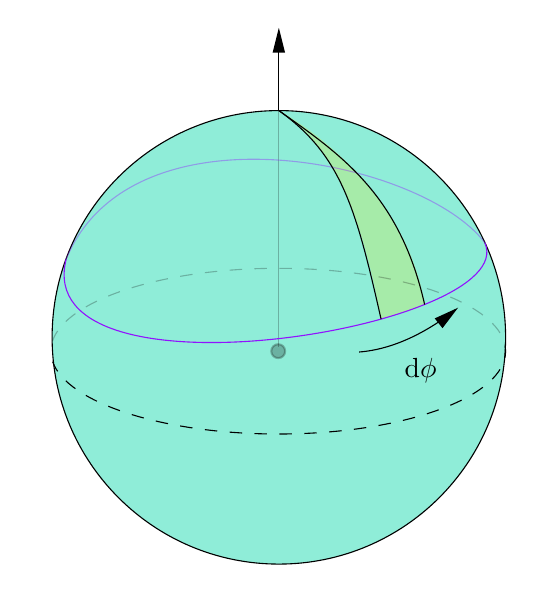
\begin{tikzpicture}[x=0.75pt,y=0.75pt,yscale=-1,xscale=1]
%uncomment if require: \path (0,300); %set diagram left start at 0, and has height of 300

%Shape: Circle [id:dp5046650378220048] 
\draw  [fill={rgb, 255:red, 80; green, 227; blue, 194 }  ,fill opacity=0.64 ] (262.21,175.75) .. controls (262.21,115.41) and (311.12,66.5) .. (371.46,66.5) .. controls (431.79,66.5) and (480.71,115.41) .. (480.71,175.75) .. controls (480.71,236.09) and (431.79,285) .. (371.46,285) .. controls (311.12,285) and (262.21,236.09) .. (262.21,175.75) -- cycle ;
%Shape: Polygon Curved [id:ds5250467240215824] 
\draw  [draw opacity=0][fill={rgb, 255:red, 184; green, 233; blue, 134 }  ,fill opacity=0.57 ] (371.46,66.5) .. controls (394.94,79.85) and (433.74,111.85) .. (441.71,159.98) .. controls (438.71,161.98) and (432.94,163.05) .. (420.71,166.98) .. controls (416.54,145.45) and (406.14,87.05) .. (371.46,66.5) -- cycle ;
%Shape: Arc [id:dp639258111017756] 
\draw  [draw opacity=0][dash pattern={on 4.5pt off 4.5pt}] (480.45,185.11) .. controls (480.62,184.23) and (480.7,183.33) .. (480.7,182.42) .. controls (480.7,160.38) and (431.66,142.5) .. (371.16,142.49) .. controls (315.32,142.48) and (269.23,157.69) .. (262.46,177.37) -- (371.15,182.41) -- cycle ; \draw  [color={rgb, 255:red, 0; green, 0; blue, 0 }  ,draw opacity=0.25 ][dash pattern={on 4.5pt off 4.5pt}] (480.45,185.11) .. controls (480.62,184.23) and (480.7,183.33) .. (480.7,182.42) .. controls (480.7,160.38) and (431.66,142.5) .. (371.16,142.49) .. controls (315.32,142.48) and (269.23,157.69) .. (262.46,177.37) ;
%Straight Lines [id:da9099277732366831] 
\draw    (371.46,28.61) -- (371.46,66.5) ;
\draw [shift={(371.46,26.61)}, rotate = 90] [fill={rgb, 255:red, 0; green, 0; blue, 0 }  ][line width=0.08]  [draw opacity=0] (12,-3) -- (0,0) -- (12,3) -- cycle    ;
%Straight Lines [id:da5824346930589386] 
\draw [color={rgb, 255:red, 0; green, 0; blue, 0 }  ,draw opacity=0.25 ]   (371.46,66.5) -- (371.46,180.53) ;
%Shape: Arc [id:dp687936282701906] 
\draw  [draw opacity=0][dash pattern={on 4.5pt off 4.5pt}] (480.45,179.7) .. controls (480.62,180.58) and (480.7,181.48) .. (480.7,182.39) .. controls (480.7,204.43) and (431.66,222.31) .. (371.16,222.33) .. controls (315.32,222.34) and (269.23,207.12) .. (262.46,187.44) -- (371.15,182.41) -- cycle ; \draw  [dash pattern={on 4.5pt off 4.5pt}] (480.45,179.7) .. controls (480.62,180.58) and (480.7,181.48) .. (480.7,182.39) .. controls (480.7,204.43) and (431.66,222.31) .. (371.16,222.33) .. controls (315.32,222.34) and (269.23,207.12) .. (262.46,187.44) ;
%Straight Lines [id:da1722555323787216] 
\draw    (262,168.95) ;
%Straight Lines [id:da03626750387054689] 
\draw [color={rgb, 255:red, 0; green, 0; blue, 0 }  ,draw opacity=0.25 ]   (371.15,182.41) ;
\draw [shift={(371.15,182.41)}, rotate = 0] [color={rgb, 255:red, 0; green, 0; blue, 0 }  ,draw opacity=0.25 ][fill={rgb, 255:red, 0; green, 0; blue, 0 }  ,fill opacity=0.25 ][line width=0.75]      (0, 0) circle [x radius= 3.35, y radius= 3.35]   ;
%Curve Lines [id:da11755103924593024] 
\draw [color={rgb, 255:red, 144; green, 19; blue, 254 }  ,draw opacity=1 ]   (269,138) .. controls (250.71,210.2) and (488.71,171.2) .. (470.71,130.2) ;
%Curve Lines [id:da05946487398733602] 
\draw [color={rgb, 255:red, 144; green, 19; blue, 254 }  ,draw opacity=0.37 ]   (269,138) .. controls (300.71,61.2) and (440.71,90.2) .. (470.71,130.2) ;
%Curve Lines [id:da02604208213784487] 
\draw    (371.46,66.5) .. controls (401.71,87.98) and (408.71,113.98) .. (420.71,166.98) ;
%Curve Lines [id:da2819669603292758] 
\draw    (371.46,66.5) .. controls (401.71,87.98) and (429.71,106.98) .. (441.71,159.98) ;
%Curve Lines [id:da37610290595360074] 
\draw    (410.1,182.83) .. controls (429.9,181.25) and (446.72,170.14) .. (456.34,162.64) ;
\draw [shift={(457.8,161.48)}, rotate = 501.33] [fill={rgb, 255:red, 0; green, 0; blue, 0 }  ][line width=0.08]  [draw opacity=0] (12,-3) -- (0,0) -- (12,3) -- cycle    ;

% Text Node
\draw (439.79,184.69) node [anchor=north] [inner sep=0.75pt]    {$\mathrm{d} \phi $};


\end{tikzpicture}

    }
    \caption{单自旋的场构型和Berry相位}
\end{figure}

自旋系统的路径积分中的Berry相位项实际上具有特殊的意义。对单独的一个自旋,其场构型的取值范围就是$\mathbb{R} / \beta \rightarrow S^2$,$\mathbb{R} / \beta$指的是虚时间,而$S^2$则是一个特定的虚时间点的$\vb*{n}$取值范围。
因此,一个特定的场构型画出来就是Bloch球上的一个有方向的闭合曲线,可以记作$\gamma$。
注意到立体角为
\[
    \dd{\Omega} = \sin \theta \dd{\theta} \dd{\varphi},
\]
半径为1的球面上,画出连接一小段路径$\dd{\vb*{r}}$上的某一点$\vb*{r}$和北极的大圆弧,则$\vb*{r}$运动时这段大圆弧扫过的面积是
\[
    (1 - \cos \theta) \dd{\varphi} = \int_0^\theta \sin \theta' \dd{\theta'} \dd{\varphi},
\]
$\dd{\vb*{r}}$的方向顺时针为负,逆时针为正。
上式左边乘以$S$正好是\eqref{eq:spin-path-integral}中的Berry相位项的微元。
将这些微元求和起来,我们会得到$S^2$上的这样一块面积,它的边界就是$\gamma$(\autoref{fig:spin-field-area})。
在南极和北极的连线和$\gamma$有交叉时,$\gamma$围成的面积存在歧义,由于我们是从$\theta=0$处开始积分,即从北极开始积分,应当认为$\gamma$围绕着北极。

我们常常将\eqref{eq:spin-path-integral}中的Berry相位项称为“拓扑项”,即定义
\begin{equation}
    S_\text{topo}[\vb*{n}] = \ii S \int_0^\beta \dd{\tau} (1 - \cos \theta) \partial_\tau \phi.
    \label{eq:single-spin-topo-term}
\end{equation}
这么说是有依据的,但是要清楚地说明为什么需要首先说明一些前置的概念。以下设
\begin{equation}
    \Gamma[\vb*{n}_i] = \int_0^\beta \dd{\tau} (1- \cos \theta_i) \partial_\tau \phi_i
\end{equation}
以简化书写。

有量子涨落的自旋链的路径积分中的一个路径是一个二维底流形到$S^2$的映射,其中一维是虚时间,另一维是离散的格点坐标,即场构型的取值范围就是$N \times (\mathbb{R} / \beta) \to S^2$,在自旋非常多时,就会得到$\mathcal{M} \times (\mathbb{R} / \beta) \to S^2$,其中$\mathcal{M}$是系统占据的一维空间。
不做任何粗粒化时$\mathcal{M} \times (\mathbb{R} / \beta)$是一系列圆圈的并集,每个圆圈是固定一个格点,$\tau$从$0$演化到$\beta$的路径;将空间粗粒化,$\mathcal{M} \times (\mathbb{R} / \beta)$是一个圆柱面,其轴是空间坐标$x$轴。
然而还应该注意到,我们通常会认为空间无穷远处什么过程都不会发生,从而在$x = \pm \infty$处可以认为没有时间演化,$\tau$恒定为零,从而实际上可以将圆柱的两端——$x = \pm 1$处——“封起来”,将圆柱变成$S^2$。
也即,一维自旋链的底流形实际上可以看成$S^2$。容易看出$(\tau, x)$坐标系正是经纬度,$\tau$是经度而$x$是纬度。

假定一个反铁磁序能够生成。我们可以做分解
\begin{equation}
    \vb*{n}_i = (-1)^i \vb*{\phi}_i + \vb*{m}_i,
\end{equation}
其中$\vb*{\phi}_i$是反铁磁序序参量而$\vb*{m}_i$是铁磁序序参量,后者远远小于前者。
请注意此时$\vb*{\phi}_i$和$\vb*{m}_i$的具体定义并没有唯一确定——我们只需要$\vb*{\phi}_i$远大于$\vb*{m}_i$,且两者在晶格常数$a \to 0$时形成的连续场足够光滑即可。
由于$\abs{\vb*{n}_i} = 1$总是成立而$\vb*{n}_i$中$\vb*{\phi}_i$占据压倒性地位,假定$\abs{\vb*{\phi}} = 1$恒成立总是可以的:此时$\vb*{\phi}_i$确实远大于$\vb*{m}_i$,
不过为了方便起见,我们首先重新定义$\vb*{n}$,做代换
\begin{equation}
    \vb*{n}_i \longrightarrow (-1)^i \vb*{n}_i,
    \label{eq:spin-chain-daggering-configuration}
\end{equation}
则
\begin{equation}
    \vb*{n}_i = \vb*{\phi}_i + (-1)^i \vb*{m}_i.
    \label{eq:spin-chain-afm-decomposition-after-staggering}
\end{equation}
在变换\eqref{eq:spin-chain-daggering-configuration}下
\[
    \sum_i JS^2 \vb*{n}_i \cdot \vb*{n}_{i+1} \longrightarrow - JS^2 \sum_i \vb*{n}_i \cdot \vb*{n}_{i+1},
\]
而
\[
    - JS^2 \int \dd{\tau} \sum_i \vb*{n}_i \cdot \vb*{n}_{i+1} = \frac{JS^2}{2} \int \dd{\tau} \sum_i (\vb*{n}_{i+1} - \vb*{n}_i)^2 + \const.
\]
Berry相位项在\eqref{eq:spin-chain-daggering-configuration}作用下则是
\[
    \sum_i \ii S \Gamma[\vb*{n}_i] = \ii S \sum_{\text{odd $i$}} (\Gamma[\vb*{n}_{i+1}] + \Gamma[\vb*{n}_i]) \longrightarrow \ii S \sum_{\text{odd $i$}} (\Gamma[\vb*{n}_{i+1}] + \Gamma[-\vb*{n}_i]) ,
\]
通过简单的几何分析可以看出,
\begin{equation}
    \Gamma[-\vb*{n}] = 4 \pi - \Gamma[\vb*{n}] = - \Gamma[\vb*{n}] + \const,
\end{equation}
常数$4 \pi \ii$在配分函数中不会有任何贡献。既然只考虑反铁磁序而忽略其上的铁磁涨落,Berry相位项之和为
\[
    \ii S \sum_\text{odd $i$} (\Gamma[\vb*{n}_{i+1}] - \Gamma[\vb*{n}_i]),
\]
即它是Bloch球上的曲线$\vb*{n}_{i+1}: S^2 \to S^2$围绕Bloch球北极的面积减去$\vb*{n}_i : S^2 \to S^2$围绕Bloch球北极的面积。
因此在变换\eqref{eq:spin-chain-daggering-configuration}下,$\vb*{n}$的作用量为
\begin{equation}
    S = \ii S \int \dd{\tau} \sum_\text{odd $i$} (\Gamma[\vb*{n}_{i+1}] - \Gamma[\vb*{n}_i]) + \frac{JS^2}{2} \int \dd{\tau} \sum_i (\vb*{n}_{i+1} - \vb*{n}_i)^2.
    \label{eq:discrete-heisenberg-spin-chain-action}
\end{equation}

如果将$\vb*{n}$场构型连续化,就有
\[
    - \int \dd{\tau} \sum_i JS^2 \vb*{n}_i \cdot \vb*{n}_{i+1} = JS^2 a \int \dd{\tau} \int (\partial_x {\vb*{n}})^2,
\]
而根据几何意义,Berry相位项做连续化后得到
\[
    {\ii S} \sum_{\text{odd $i$}} (\Gamma[\vb*{n}_{i+1}] - \Gamma[\vb*{n}_i]) \longrightarrow \ii S \frac{1}{2a} \int \dd{x} \vb*{n} \cdot (\partial_x \vb*{n} \times \partial_\tau \vb*{n}). 
\]
但是我们没有这样做,因为$\vb*{n}$中包含在空间维度上快速变化的铁磁序参量$\vb*{m}_i$,它的空间导数并不光滑,因此不能直接做连续化。
不过,我们仍然可以写出
\begin{equation}
    {\ii S} \sum_{\text{odd $i$}} (\Gamma[\vb*{n}_{i+1}] - \Gamma[\vb*{n}_i]) \longrightarrow \ii S \sum_\text{odd $i$} \vb*{n}_i \cdot ((\vb*{n}_{i+1} - \vb*{n}_i) \times \partial_\tau \vb*{n}_i). 
\end{equation}
我们将\eqref{eq:spin-chain-afm-decomposition-after-staggering}代入\eqref{eq:discrete-heisenberg-spin-chain-action},则
\[
    \begin{aligned}
        \ii S \sum_\text{odd $i$} (\Gamma[\vb*{n}_{i+1}] - \Gamma[\vb*{n}_i]) &\approx \ii S \sum_\text{odd $i$} \vb*{n}_i \cdot ((\vb*{\phi}_{i+1} - \vb*{\phi}_i - 2 \vb*{m}_i) \times \partial_\tau \vb*{n}_i) \\
        &\approx \ii S \sum_\text{odd $i$} \vb*{\phi}_i \cdot ((\vb*{\phi}_{i+1} - \vb*{\phi}_i - 2 \vb*{m}_i) \times \partial_\tau \vb*{\phi}_i) \\
        &\approx \ii S \frac{1}{2a} \int \dd{x} \vb*{\phi} \cdot ((\partial_x \vb*{\phi} - 2 \vb*{m}) \times \partial_\tau \vb*{\phi}),
    \end{aligned}
\]
第一个约等号来自$\vb*{m}_i$本身变化不很迅速的假设,第二个等号是小量近似,即$\vb*{m}_i$和$\partial_x \vb*{\phi}$都很小,从而只保留一阶小量,即丢弃$\vb*{n}$和$\partial_\tau \vb*{n}$因子中的$\vb*{m}$成分。
另一方面,有
\[
    \sum_i (\vb*{n}_{i+1} - \vb*{n}_i)^2 = 
\]

综上,反铁磁一维海森堡自旋链的低能有效理论是
\begin{equation}
    S = \underbrace{\ii \frac{S}{2} \int \dd{x} \dd{\tau} \vb*{\phi} \cdot (\partial_x \vb*{\phi} \times \partial_\tau \vb*{\phi})}_{S_\text{topo}} + \underbrace{\int \dd{x} \dd{\tau} (\partial_x \vb*{\phi})^2}_{S_0},
\end{equation}
其中$S_\text{topo}$称为\concept{Wess-Zunimo-Witten(WSW)项},它就是\eqref{eq:single-spin-topo-term}对所有自旋自由度求和的结果,且正好给出$\vb*{\phi}: S^2 \to S^2$“覆盖底流形$S^2$的面积”。
注意到
\[
    \pi_2(S^2) = \mathbb{Z},
\]
$S_\text{topo}$实际上将不同的场构型按照第二同伦群划分成了不同的同伦等价类。
这就是我们将\eqref{eq:single-spin-topo-term}称为“拓扑项”的原因:它对所有自旋自由度求和之后真的就是场构型的一个拓扑不变量。
设场构型$\vb*{\phi}$在$\pi_2(S^2)$中被分类到了$W$上,或者说它的卷绕数为$W$,或者说它覆盖底流形$S^2$的面积是$4 \pi W$,则对这样的构型
\begin{equation}
    S_\text{topo} = 2 \pi S W \ii.
\end{equation}
由此可以看出,对整数自旋的反铁磁海森堡自旋链,拓扑项是平庸的:虽然$S_\text{topo}$能够给出场构型在$\pi_2(S^2)$中的分类,但是它不会影响场构型的权重。
但半整数自旋的反铁磁海森堡自旋链中的拓扑项是非平庸的,这类系统的低能有效理论是
\begin{equation}
    Z = \int \fd{\vb*{\phi}} (-1)^W \ee^{- S_0[\vb*{\phi}]}.
\end{equation}

\begin{back}{拓扑量子场论和同伦群}{topo}
    设$M$是底流形,$T$是目标空间(即底流形上某一点处场值的取值范围),两者均为拓扑空间,一个场构型就是一个$M \to T$的连续函数。
    一个物理理论可以写成这样的形式:
    \[
        Z = \int_{\phi \in (M \to T)} \fd{\phi} \ee^{\ii \int_{x \in M} \dd{x} \mathcal{L}[\phi]}.
    \]

    大部分情况下,$S[\phi]$在场构型$\phi$有小的局域变动时也会跟着变动,从而给出非平凡的运动方程。
    不过有一些特殊的$S[\phi]$是场构型$\phi$的拓扑不变量,场构型发生小的变动,它是不变的。
    这样的作用量无法给出非平庸的动力学,但是它能够给按照它划分的不同拓扑等价类赋予不同的权重,从而仍然有物理意义。
    这种实际上是在计算拓扑不变量的量子场论称为\concept{拓扑量子场论}。

    最为“细致”的拓扑分类当然是同胚,但是使用一个形式很简洁的拓扑不变量大抵是无法做到这么细致的分类的。拓扑量子场论中的等价类通常都精确不到同胚的级别。
    一种常见的等价类划分方式为\concept{同伦}。设$\phi_1, \phi_2$是两个$M \to T$的场构型,如果存在连续映射
    \[
        f: [0, 1] \times M \to T
    \]
    使得$f(0) = \phi_1, f(1) = \phi_2$,我们说$\phi_1$和$\phi_2$同伦。直观地看,如果能够有一个超然于$M$\emph{以外}的连续时间演化过程能够将$\phi_1$转化为$\phi_2$,那么两者是同伦的。
    如果$\phi_1$和$\phi_2$同伦,那么它们一定同胚,但是反之不然。例如,字母X和Y是同伦的,但是它们不同胚。
    同伦允许“高维对象缩成更低维的”等等,而同胚则有更多的限制。
    
    依据同伦的概念可以定义\concept{同伦群},$M$的$n$阶同伦群$\pi_n(M)$是$S^n$到$M$的保持某个基点不动的映射的同伦分类。
    其群乘法通过
    \begin{equation}
        (\phi_1 * \phi_2)(x_1, x_2, \cdots, x_d) = \begin{cases}
            \phi_1(2 x_1, x_2, \cdots, x_d), \quad x_1 \in [0, 1/2], \\
            \phi_2(2 x_1 - 1, x_2, \cdots, x_d), \quad x_1 \in [1/2, 1]
        \end{cases}
    \end{equation}
    定义。
\end{back}

可以看到,一维海森堡自旋链中的量子涨落实际上是非常强烈的,以至于在一维实际上根本无法形成反铁磁序。
如果$S$是整数则拓扑项无贡献,有能隙;Haldane猜想。 % TODO

\section{ALKT链}

我们将两个相邻格点的自旋处在一个自旋单态中这件事称为一个\emph{共价键}(valence bond)。
有这个说法是因为,虽然我们这里在研究自旋模型,没有轨道自由度,也没有成键、反键,但是实际系统中,如果两个电子形成化学键,它们的轨道部分应该倾向于是对称的(否则不存在电子云交叠),从而自旋部分应该是反对称的,即自旋形成自旋单态。
因此,如果一个自旋模型中的自旋自由度可以直接追溯到单个的电子上,那么相邻格点处的自旋处在自旋单态中就意味着很可能实现这个自旋模型的实际体系中在这对格点处存在共价键。

The theorem and the boundary of a topological state look quite alike, and this is not coincidence.

spin-1/2 edge of a spin AKLT chain